\chapter{Model-based Development}\label{chap:model_based_development}
This chapter will give an introduction to some of the terms and ideas surrounding MDE. We will give an introduction to the concept of \emph{language workbenches} and demonstrate a few of the leading products on the market today. In the end we show what features the DPF Editor has to offer, and perform a comparison between all the products.

\section{Model-driven Engineering}
In the last decades we have seen a dramatic increase in software complexity. This complexity has been handled by more expressive and improved general programming languages, but has failed to keep up with the vast increase in functionality. The consequence of this is that developers are struggling to learn to new platforms, and often only learning a subset of what it has to offer. Another problem is that the developer misses the big picture, and forgets system-wide issues such as performance. MDE can help fight these issues with a higher level of abstraction. This abstraction yields advantages such as increased productivity, code quality/consistency and improved communication with domain experts, as well as programmers~\cite{rutle_thesis_2010}\cite{fowler2010domain}.

Model-driven engineering is a model-centric approach to software development, using models as first-class entities. This is in contrast to the classic code-centric approach, where models sometimes are used for describing design and is implemented by code, or the code \emph{is} the design and the implementation (agile principle). The MDE process defines models which capture the concepts of certain parts in a computer system and some kind of transformation which makes it understandable by a computer. The models need to have a narrow focus on the problem domain to reach its full potential. If the models are too general, it will become very hard to create an expressive model transformation. 
% and you could probably use a general modeling language like UML instead.

Models can be categorized as \emph{prescriptive} or \emph{descriptive}. A prescriptive model gives a description of the system before it is produced and works as a blueprint, while a descriptive model works as documentation for the system that is created~\cite{Gonzalez-Perez:2007:MSD:1290192.1290209}. In MDE, models act as both descriptive and prescriptive in the sense that the model is a replacement for the traditional code, and it also acts as a guide for understanding the system at a higher level.

\subsection{Domain-Specific (Modelling) Languages}\label{subsec:dsml}
\subsubsection{Domain-Specific Languages}
There are different ways to create a model in MDE, but in common is the need for a language in which you can specify models. A popular approach, which is often not regarded as MDE, is the creation of textual \emph{domain-specific languages} (DSL). These languages have the trait of focusing on a particular domain, where their source files acts as the model. DSLs has been used for a number of years, and are used in everything from software build tools (e.g. Ant~\cite{apache_ant}) to HTML and SQL.
Fowler~\cite{fowler2010domain} defines a few key elements for a DSL:
\begin{description}
  \item[Programming language:] A DSL is not a \emph{general programming language}, but it shares a lot of properties; it should be formal to be understood by a computer, but also be intuitive for a human being.
  \item[Language nature:] A DSL should not consist of separate expressions, but have a syntax that can be composed by several expressions put together.
  \item[Language expressiveness/focus:] The language should only support the absolute minium of features needed for a limited part of a system. The expressiveness of a good DSL comes from a clear focus on a limited domain.
\end{description}

A DSL usually consists of a grammar (that defines the language), a parser (which conforms to the grammar) and a \emph{semantic model}. Fowler defines the semantic model as "the model that is populated by a DSL", i.e. one directly populate a framework or API.\newline

\begin{figure}[h]
    \centering
    \centerline{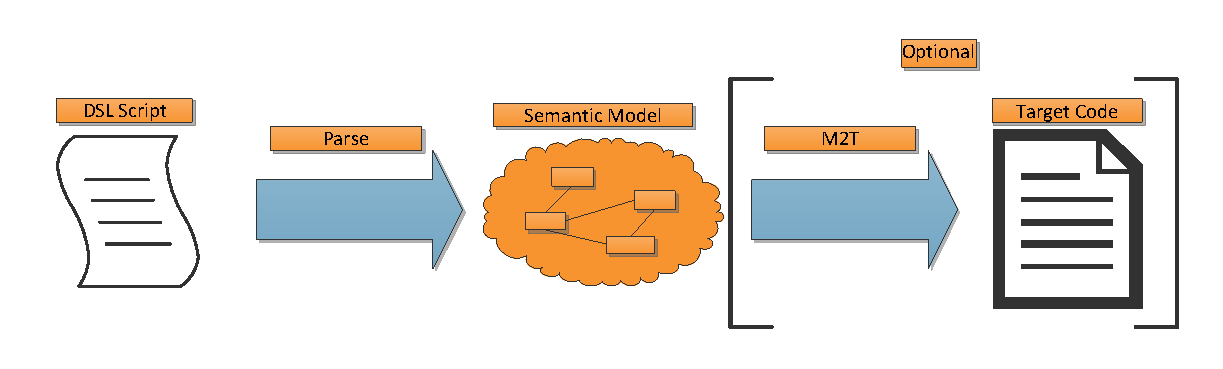
\includegraphics[scale=0.65]{images/dslm2t.pdf}}
    \caption[Domain Specific Language concept]{Figure shows how a DSL works.}
    \label{fig:dslm2t}
\end{figure}
\newpage
Figure \ref{fig:dslm2t} shows how a typical DSL works. Usually a DSL script is parsed and used to populate a semantic model which defines the semantics behind the script. As shown, model-to-text transformations are an optional part of DSLs. This is because DSLs are often used to allievate the configuration of a piece of software, and can be regarded as a thin wrapper around an API. Such DSLs are not necessarily focused on raising the level of abstraction, but rather to create a more convenient syntax for an API. In a MDE context, we want to raise the level of abstraction and provide the concrete semantics through model transformations.

Fowler~\cite{fowler2010domain} lists four main types of domain-specific languages:
\begin{description}
  \item[Internal DSLs] Internal DSLs are languages which are created within the host programming language. The host language is formed in a way that create a fluent syntax.
  \lstset{language=Java,caption=Simple internal DSL for creating specifications in DPF,label=list:internaldslexample,captionpos=b}
%   \begin{table}[ht]
%     \centering
  \begin{lstlisting}[showstringspaces=false]
builder
  .specification()
    .graph("m1")
      .node("DomainClass")
      .node("Type")
      .arrow("Attribute", "DomainClass", "Type")
      .arrow("Reference", "DomainClass", "DomainClass")
    .endgraph()

  .specification()
    .typeGraph("m1")
      .graph("instance")
	.node("Post", "DomainClass")
	.node("User", "DomainClass")
      .endgraph()
  \end{lstlisting}
%   \end{table}
  Listing \ref{list:internaldslexample} shows a simple internal DSL created in Java for populating a DPF model. This particular example uses \emph{method chaining}, a technique where a method (e.g. node()) returns its class instance when called.
  
  \item[External DSLs] External DSLs are the most common DSLs. These languages use external DSL scripts which are not bound be the host language's syntax and thus have a lot more syntactic freedom. Text files are parsed and used to either populate a semantic model, or do a model transformation (see figure \ref{fig:dslm2t}). Examples of such languages are SQL, HTML, XAML, Make etc.
 \lstset{caption=External DSL for creating specifications in DPF,label=list:externaldslexample,captionpos=b}
%   \begin{table}[ht]
%     \centering
    \begin{lstlisting}[showstringspaces=false]
mm:=TGraph<DPF>{
  z:Node-e0:Arrow->b:Node,
  a:Node-e1:Arrow->b:Node-e2:Arrow->c:Node-t:*->String,
}

m:=TGraph<mm>{
  b:c-y@1:t->["Hallo"],
  b:c-y@2:t->["Test"],
  f:a-l:e1->o:b,
}

ecore(mm)
    \end{lstlisting}
%   \end{table}
  Listing \ref{list:externaldslexample} shows an external DSL for defining \emph{DPF specifications}\footnote{The textual DPF tool is part of Florian Mantz' Ph.D. work.}. This example shows model \codeText{m} being typed by a metamodel \codeText{mm}, and then serializing the model. DPF is explained in section~\ref{sec:dpf}.
  \item[Fragmentary DSLs] These are DSLs which are embedded in the host programming language, such as \emph{regular expressions}.
  \item[Language workbenches] Discussed in section~\ref{sec:language_workbenches}.
\end{description}

\subsubsection{Domain-Specific Modelling Languages} 
DSMLs serve the same purpose as a DSL, but is usually presented in a visual manner. These languages are specified according to a \emph{metamodel}, sometimes defined as a "model of models"~\cite{rutle_thesis_2010}. The DSMLs are usually defined by domain experts and experienced developers to ensure that the domain concepts are properly described. The languages are then used by other developers as a programming tool. These languages are dependent on surrounding functionality and tooling, e.g. graphical editors, code generators and model validation. Workflow and tooling are further discussed in section~\ref{sec:language_workbenches}, Language Workbenches. 
\begin{figure}[htpb]
    \centering
    \centerline{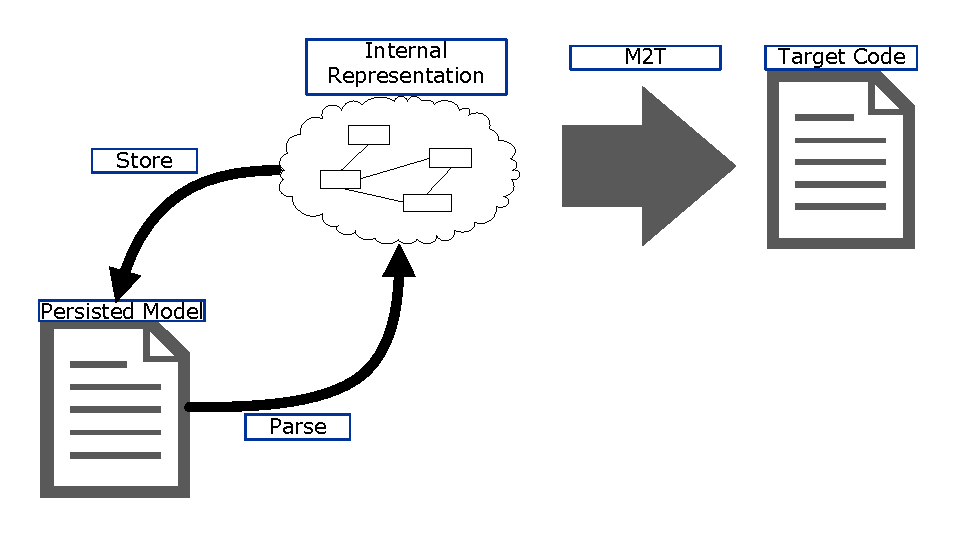
\includegraphics[scale=0.7]{images/dsml2.pdf}}
    \caption[Domain Specific Modelling Language tool]{An abstract view of a Domain Specific Modelling Language tool.}
    \label{fig:dsml2}
\end{figure}

The main difference between DSLs and DSMLs are the inner workings of the modelling environment. Both DSLs and DSMLs needs a parser which can translate the source file to an internal representation. The DSL's parser usually produce an abstract syntax tree or it populates a semantic model. 

Figure \ref{fig:dsml2} shows how the equivalent of the DSL script is the internal representation in a DSML-tool. The internal representation of the model is the model; the persisted model are only a means for the computer to understand the model. The model-to-text transformation (M2T) is not marked as optional as in figure \ref{fig:dslm2t}, because DSMLs require some kind of model transformation to have any meaning to a computer. 

The DSML is dependent on tooling, e.g. a visual editor which has an internal representation of the model. Usually this model also has an external representation in the form of a file. A popular format for this is the XML Metadata Interchange (XMI), a XML-based format that is tailored for representing models. Furthermore DSMLs are purely a MDE concept, and are rarely used to populate semantic models.
Model transformations with DSLs and DSMLs are discussed further in chapter~\ref{chap:code_generation}.

% Ein figur som viser DSML(persistence) -> parsing -> inner representation/semantic model -> m2t/m2m
% Ta med noko om korleis ein DSML er representert innad i verktøy

%that DSLs are constrained by a grammar that defines the language. This grammar is centered around the key concepts of a domain. 
% A DSML uses a base language in which you specify your metamodel(s) that in its turn defines the key concepts in the domain. 

% - dslar mot dsml \newline MOAR?

\subsection{Model-driven Architecture}
Model-driven Architechture is the Object Management Group's (OMG)~\cite{MDA} model-driven development initiative and can be regarded as a predecessor to MDE. It was launched as a standard in 2001. Even though the concepts of domain-specific modelling was known, OMGs MDA created new interest in the subject. Its core principle is to abstract away technology details of a specified system with the use of platform-independent models (PIM). PIMs contain business functionality and behaviour, and are reusable across any operating system/architecture. Before generating any code from a MDA project to a target environment, a platform-specific model (PSM) is created through \emph{model-to-model transformations}. A PSM is generated for each target environment. 
\begin{quote}
``The primary goals of MDA is portability, interopability and reusability through architectural separation of concern.~\cite{MDA}''
\end{quote}
MDA meets a lot of critique for different reasons. MDA uses model-to-model transformations to generate more detailed models as you go, i.e. from a PIM to a PSM resulting in the need to maintain more models than necessary. Another problem arise when you edit the PSM; how is this reflected in the PIM?

The MDA spec is centered around OMG's own standards. The modelling language used is very often UML, but it can be any \emph{Meta-Object Facility (MOF)} compliant modelling language. MOF is a closed metamodel hierarchy with four levels (see more in next section).

\section{Metamodelling}
Metamodelling is an important concept in MDE, yet its definition is highly debated~\cite{rutle_thesis_2010}~\cite{rossini_thesis_2011}. A metamodel is sometimes referred to as a "model of models"; Cook and Kent~\cite{cook:domainspecificide} claims this is a bad definition and should rather be ``a model of the concepts expressed by a modelling language''. A suitable definition could also be ``a model of a modelling language''. 

\begin{figure}[h]
    \centering
    \centerline{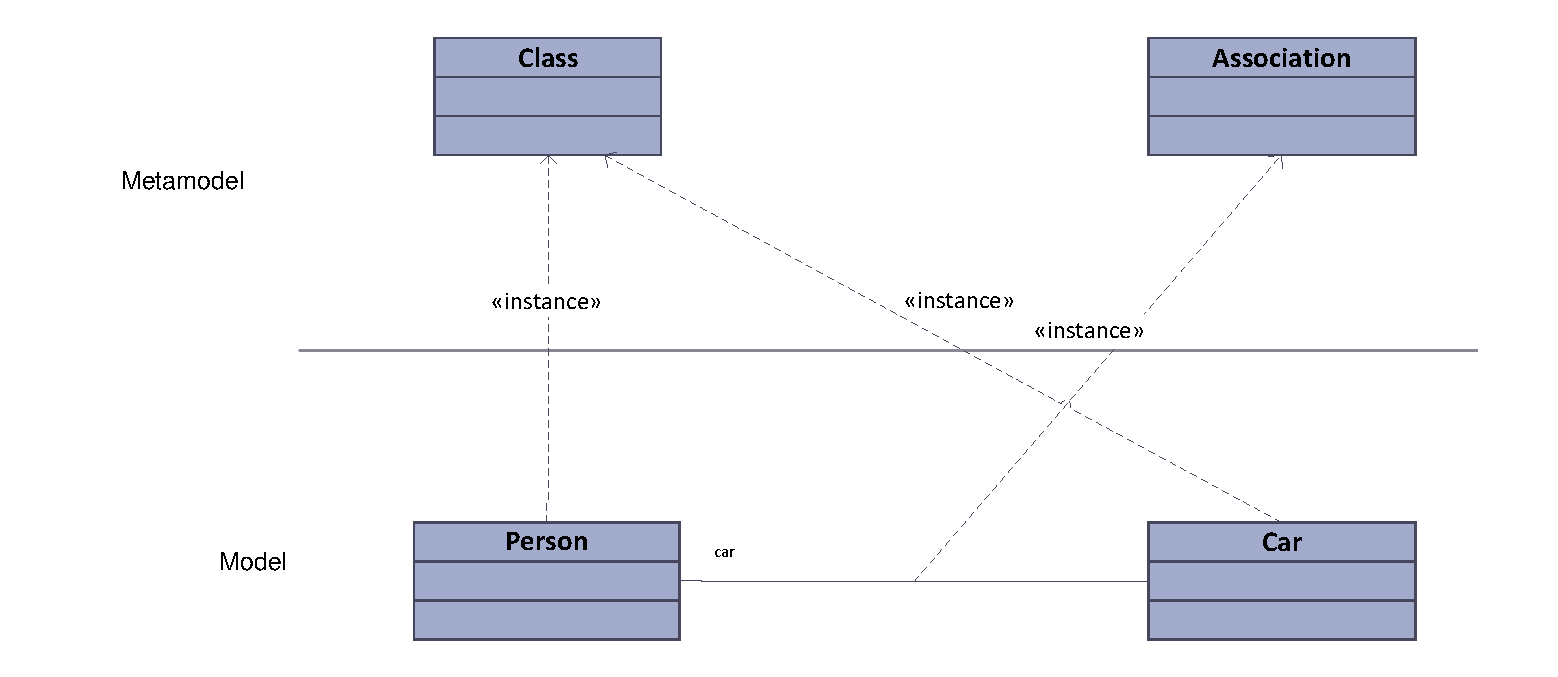
\includegraphics[scale=0.6]{images/uml_metamodel_example.pdf}}
    \caption[UML metamodel example]{A simple metamodel/model example.}
    \label{fig:uml_metamodel_example}
\end{figure}

Figure \ref{fig:uml_metamodel_example} shows a simple metamodelling example where each of the modelling constructs is an instance of a concept from the metalevel. A metamodel specifies the abstract syntax of a modelling language. This syntax defines the concepts, attributes, their relationships and how they fit together to create a valid model~\cite{rutle_thesis_2010}. A model's available features is defined by what features its metamodel defines. Metamodels has their own \emph{meta-metamodel} which define the syntax they must adhere to as well. The metalayer on top of the hierarchy is usually defined by a \emph{reflexive} modelling language, a language which is defined in itself.

In 1997 OMG adopted MOF 1.1 as a standard, around the same time as UML 1.1 was adopted. The goal of MOF is to create a common way of describing model metadata (data about models). This is done through a number of specifications such as MOF Core, MOF IDL Mapping, MOF XMI Mapping, MOF Model to text (MOFM2T) among others.

\begin{figure}[htpb]
    \centering
    \centerline{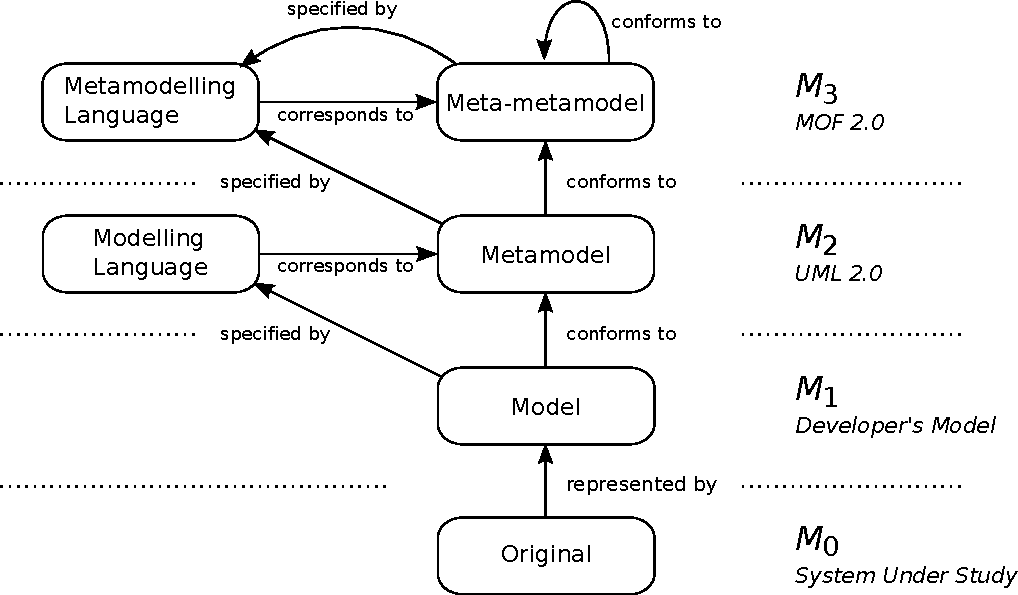
\includegraphics[scale=0.5]{images/omg_hierarchy.pdf}}
    \caption[MOF hierarchy]{Figure shows the four layer hierarchy defined in MOF.}
    \label{fig:mof}
\end{figure}

MOF defines a metamodel hierarchy with four layers (M$_{3}$ to M$_{0}$) where each level conforms to the level above it. MOF's goal is to create a "grammar" for how the models should be formed. MOF has two variants; Complete MOF (CMOF) and Essential MOF (EMOF). EMOF contains only the most basic constructs, which in broad strokes is classes, relations, types, packages and operations. Even though an EMOF compliant modelling language is enough for a lot of use cases, the language is fixed and thus falls short compared to the expressiveness of a DSML created without an EMOF compliant modelling language.

Figure \ref{fig:mof} shows that the M$_{3}$ level, the meta-metamodel, is defined in itself (\emph{reflexive layer}). This is done through constructs which the MOF specification provides. This layer is the metamodel for the UML language. The M$_{2}$ level is the instance of M$_{3}$, and is the model which implements UML, adhering to the abstract syntax of the layer above. The M$_{1}$ layer is where UML concepts such as Class, Atttribute and Operations are used to create a comprehensible model of the system which is then instantiated by level M$_{0}$, the \emph{system under study (SUS)}. M$_{0}$ contains the original, real world object, e.g. "Ford" would be instance of a M$_{1}$ class Car.

MOF is often under criticism in the literature for beeing, rigid because of a fixed number of metalevels (MOF is sometimes referred to as the four-layered hierarchy). This criticism is somewhat incorrect as the MOF specification does not restrict the number of layers~\cite{OMG07UML}. %7.12 i uml ref

% - Why several layers -> abstraction
% - fleirnivå grafisk modellering

\section{Constraints}
A constraint helps us to specify complex requirements beyond what basic modelling constructs can offer. In UML we have the option to apply constraints to our models. Unfortunately only simple constraints like multiplicity and uniqueness can be applied directly in the metamodel. These constraints are called \emph{structural constraints}. If we want to create a constraint which cannot be declared in the model, we need to create these externally. 

The "external" constraints are called \emph{attached constraints}, and are created using a declarative language like \emph{Object Constraint Language (OCL)}~\cite{OMG06OCL}. A solution like this is problematic; a UML model is a graph based model and OCL is textual language, making it harder to reason about the models. Not only for the developer, but also for the domain expert(s). There are also issues with reflecting changes in the model against the OCL constraints, creating synchronization issues~\cite{rutle_thesis_2010}. OCL is an OMG standard and is the recommended attached constraints facility used in combination with UML and MDA. 

\section{Language Workbenches}\label{sec:language_workbenches}
Language workbench is a term coined by Martin Fowler~\cite{fowler2010domain} that describes an environment for creating DSML/DSLs and corresponding tools. The workbenches should provide an IDE-like environment for creating DSML/DSLs, and in addition to generate code it should generate tooling for the specified language. Language workbenches are a relatively new concept which has been increasingly popular the last few years, and is under heavy research and changes. 
When working with language workbenches, the development process are divided into two phases. Figure~\ref{fig:lwusecase} shows how the DSML is created along with relevant tooling, such as editors and code generators. This activity should be performed by domain experts, as well as developers with experience. Using experienced developers will ensure that the tooling for the language is tailored to the users (which are developers). The figure also illustrates that developers utilize the domain-specific environment created from the DSML. \newline
\begin{figure}[hp]
    \centering
    \centerline{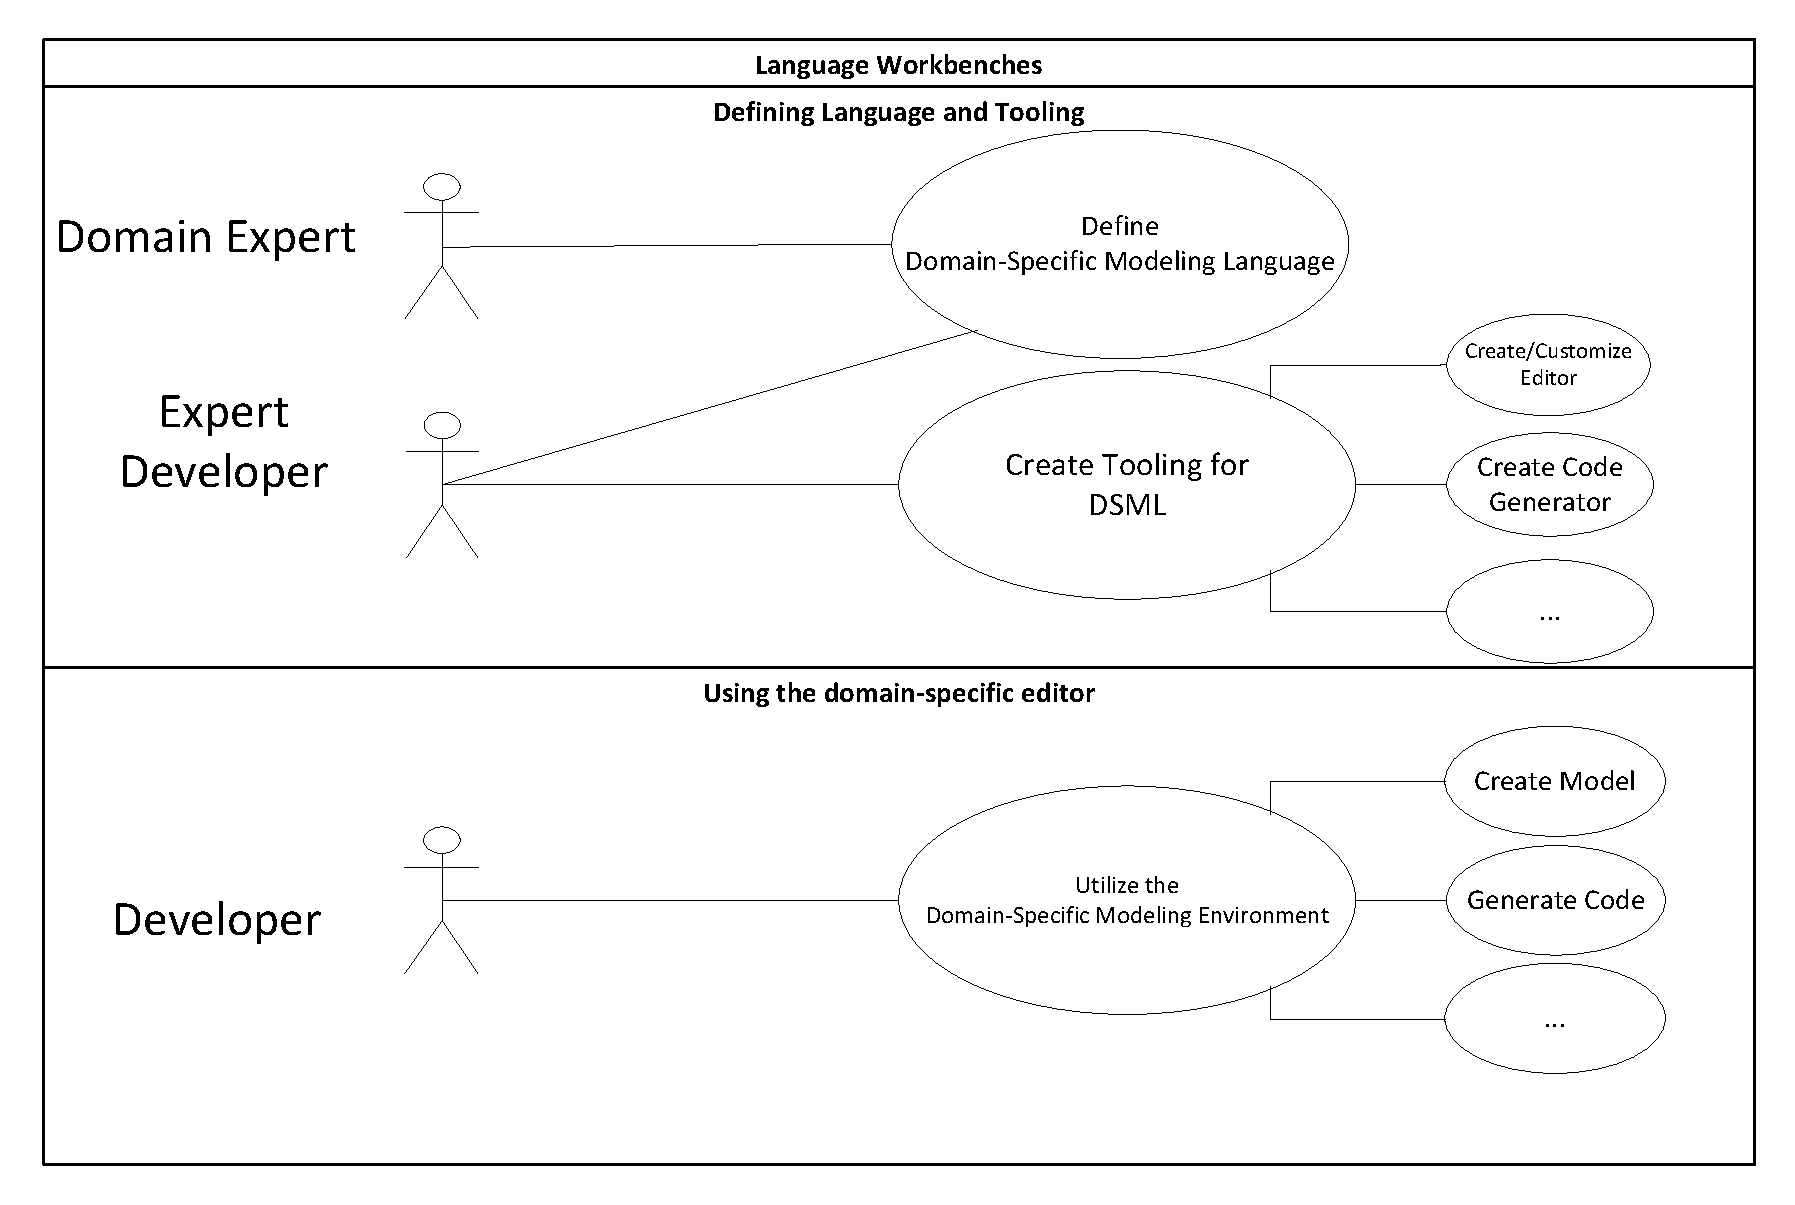
\includegraphics[scale=0.5]{images/LanguageWorkbenchUseCase.pdf}}
    \caption[Language workbench workflow]{Figure shows the intended workflow for a language workbench.}
    \label{fig:lwusecase}
\end{figure}

Martin Fowler describes a few common elements in a language workbench~\cite{fowler2010domain}:
\begin{description}
  \item[\emph{Semantic Model} schema] defines the structure of the \emph{Semantic Model}, based on a metamodel. In language workbenches the semantic model is the metamodel used for the model. Fowler uses the term \emph{schema} for the metamodel, or DSML if you like. The base model of the tool is called a \emph{schema definition language}.\newpage
  \item[DSML editing environment] defines an IDE-like experience when editing a DSML/DSL, often through \emph{projectional editing}.
  Projectional editing provides some kind of interface where we edit our models. Besides the diagrammatic approach, there are also schemas, forms, hierarchies etc. The counterpart of projectional editing is source editing, which is traditional programming using text files. Some language workbench solutions gives the opportunity of using multiple projections for your model, i.e. you can get a schema representation of a diagram based model, or a text representation.
  \item[Semantic Model behaviour] defines the semantics of the language specified. Usually this is achieved through code generation.
  Although the model is stored in the language workbench, the computer does not understand the intent of the model initially. The semantics of a DSML is defined through model transformations. The model can configure an API, create an interpreter, do a model-to-model transformation, but most often generating executable code (model-to-text transformation) is the chosen solution.
\end{description}

\begin{figure}[htpb]
    \centering
    \centerline{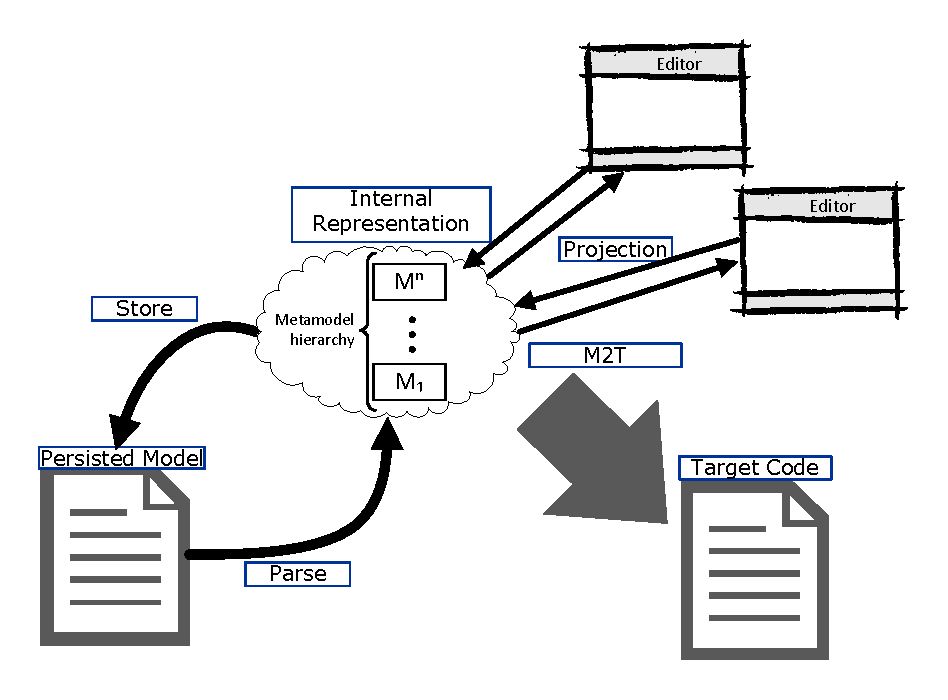
\includegraphics[scale=0.8]{images/dsml3.pdf}}
    \caption[Language workbench]{Figure shows a conceptual view of a language workbench.}
    \label{fig:dsml}
\end{figure}

Figure \ref{fig:dsml} shows how a language workbench work conceptually. At the heart of the language workbench, we find an internal representation of any models we operate on. This might be a single model, or a complete metamodel hierarchy. It forms the basis for the tools built around it. The tooling in a language workbench is defined as anything from the concept of a schema-definition language to code generators and constraint validation. The figure shows the most basic parts needed for a functional language workbench. As discussed in section~\ref{subsec:dsml} the internal representation of the model is the model. A persistence facility is needed for reuse and storing of the models. The persisted version of the models are not meant for hand editing, this should be done through the editing environment. 

% Rich tooling can enhance the modeling experience, but.

% In contrast to figure \ref{dslm2t} we see some differences; the equivalent of the DSL script is the internal representation of a DSML where persistence of the model is only used because we want the model to exist beyond the memory of a computer. The model is often stored in XMI, and is not made for handediting.
% MODELL SOM VISER KORLEIS SCHEMA LANG-> METAMODELL ->MODELL
% Figure [lol] shows 
% Along with tools like Obeo Designer and MetaEdit+, we find that DPF Editor fits these critera and introduces a new approach to domain-specific modeling. //MEH\newline
% define tooling\newline
% - Components: Model, generator, model framework/semantic model, target environment, dsm tooling, schema-definition language,\newline

\section{Existing Language Workbench Solutions} 
This section gives a brief overview of some of the more popular projection based language workbench solutions on the market today. 
% We will present some of the features of each solution.

\subsection{Eclipse and Eclipse Modeling Framework}
The Eclipse Foundation~\cite{Eclipse} is a non-profit organization which was established in 2004 with the goal of creating a vendor-neutral, transparent and open community around the Eclipse projects. The Eclipse eco-system consists of a vast amount of projects, everything from development tooling to SOA and web related projects. A common misconception is that when people think of Eclipse, they have Eclipse Java Development Tools (JDT) in mind. Eclipse JDT is a combination of different Eclipse projects, and provides a feature rich Integrated Development Environment for the Java programming language. This means Eclipse JDT is a collection of (in)dependent plug-ins which ultimately results in the IDE. The philosophy behind Eclipse is modularity; at the heart of Eclipse lies Equinox, an implementation of the OSGi core framework specification, which facilitates the modular nature of the \emph{Eclipse Platform}~\cite{eclipse_whitepaper}. All functionality in Eclipse is provided through plug-ins.

\subsubsection{EMF} \label{subsub:emf}
EMF (or rather EMF Core) is the project at the center of Eclipse's modelling technologies. The framework aims to unite Java, XML and UML; models in EMF can be expressed either way, where one can generate one representation from the other~\cite{BudinskyMerksS06}. EMF is a modelling tool which can be found in the middle of a pure modelling tool and Java code. Instead of following the "raising abstraction" mantra of pure modelling tools, EMF recognizes the need for a tool where the programmer can easily understand the mapping between model and code. EMF provides a modelling environment based on its own metamodel Ecore (which is a reflexive model). Ecore contains a basic set of modelling constructs that corresponds to EMOF. EMF also provide persistence and a code generation facility that can generate Java code from your metamodel, unit-tests for said code, and the possiblity to generate a simple hierarchy based editor. EMF does not facilitate code generation from the model instance level. This is handled by other modelling components, such as tools from the M2T (model-to-text) project.

\begin{figure}[htpb]
    \centering
    \centerline{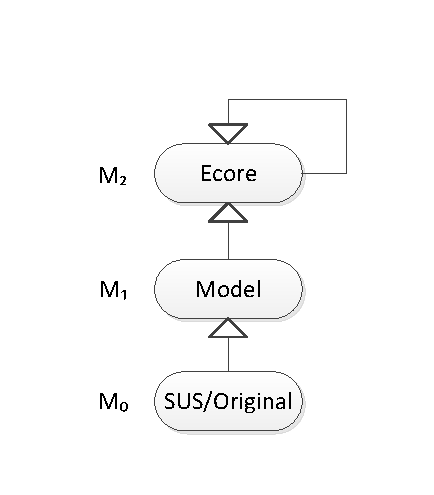
\includegraphics[scale=0.8]{images/ecoremof.pdf}}
    \caption[Ecore and MOF]{Figure shows a how Ecore fit into the MOF hierarchy.}
    \label{fig:ecoremof}
\end{figure}
Figure~\ref{fig:ecoremof} shows how Ecore fit into the MOF hierarchy. As the figure shows, EMF does not give you the possiblity of multiple metalevels. Although this restriction strengthens the intent of a comprehensible mapping between model and code, it makes it hard to create a DSML that can be substituted for code. An important note about Ecore's MOF hierarchy is that the levels vary based on what you try to achieve. With the use of the UML2 support, one have four levels as usual, but if you use Ecore to model a system directly, you only have three levels.

\begin{figure}[htpb]
    \centering
    \centerline{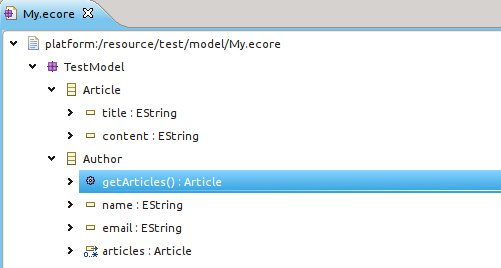
\includegraphics[scale=0.8]{images/emf_hierarchy.jpeg}}
    \caption[Creating an Ecore file]{Figure shows editing an Ecore file using the hierarchy view.}
    \label{fig:emf_hierarchy}
\end{figure}

\begin{figure}[htpb]
    \centering
    \centerline{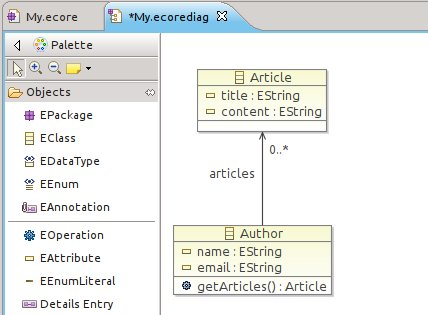
\includegraphics[scale=0.8]{images/emf_diagram.jpeg}}
    \caption[Creating an Ecore file diagramatically]{Figure shows editing an Ecore file using the graph based view.}
    \label{fig:emf_diagram}
\end{figure}

Figure \ref{fig:emf_hierarchy} and \ref{fig:emf_diagram} shows how the creation of a metamodel in Ecore. You can choose between the hierarchy solution, or a projectional view which requires the generation of an Ecore Diagram file.

EMOF defines a limited amount of modelling constructs, among them classes, attributes, references, packages and operations. These concepts are easy to understand for any programmer with a background in object oriented languages, and thus creating a clear understanding of the mapping between model and code. As the MOF standard~\cite{OMG06MOF} defines, constraints beyond cardinality and uniqueness are defined externally. In EMF one can define \emph{invariants} which are defined as a boolean method in the model, or a constraint which is defined as a method on a validator class, not in the model itself. Either way, hand editing is required to define what the constraint/invariant actually constrains. The implementations can use OCL if desired.

\subsection{Obeo Designer}
Obeo Designer is the product of a french company named Obeo. Obeo is a consulting company which has a strong focus on MDE and MDA. The company is an Eclipse Foundation Strategic Member and a contributor on many Eclipse Modelling projects. Obeo Designer is based on Eclipse EMF, which means it uses \emph{Ecore} as its modelling language. The tool's main focus is on creating visualizations for your model, as well as generators. 

\begin{figure}[hp]
  \centering
  \centerline{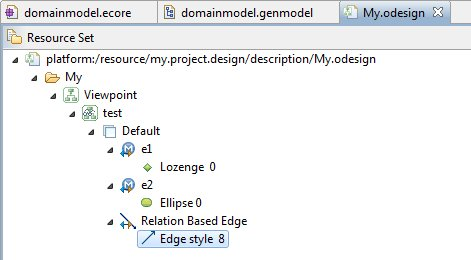
\includegraphics[scale=0.8]{images/obeo_graph_example.jpeg}}
  \caption[Creating graphs in Obeo Designer]{Example of creating a custom visualization for an Ecore model in Obeo Designer.}
  \label{fig:obeo_graphvisual}
\end{figure}

\begin{figure}[hp]
  \centering
  \centerline{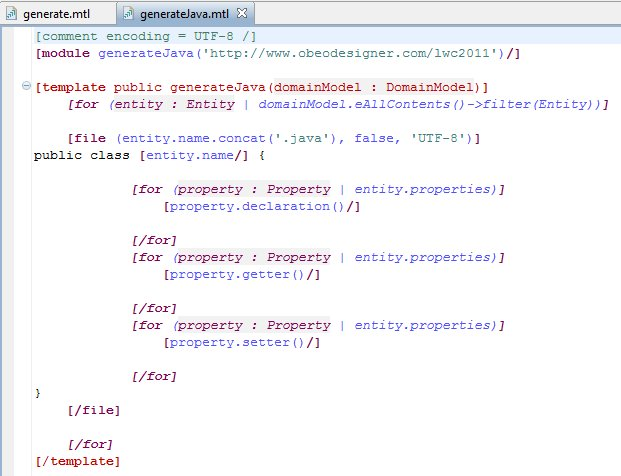
\includegraphics[scale=0.7]{images/obeo_generate_code.jpeg}}
  \caption[Creating templates using Acceleo]{Creating Acceleo templates for code generation.}
  \label{fig:obeo_code}
\end{figure}

Figure \ref{fig:obeo_graphvisual} shows the editor for creating custom visualizations for your Ecore model. There is no graphical editor for creating graphics, one have to choose from a set of pre-defined ones or use an external image. 

\newpage

One of the promoted features of Obeo Designer is the option of creating layers in your graph visualizations. This means you can create visualizations which fulfill a certain criteria. Take a family tree (a simple hierarchy) DSML as example; if we detect that two people are cousins, we can create a visualization that shows this by placing an arrow between them or similar.
% [set inn bilete med og utan layer] ?

Figure ~\ref{fig:obeo_code} shows Obeo's own code generation facility Acceleo~\cite{acceleo}. Acceleo is further reviewed in section~\ref{subsec:acceleo}.

Obeo Designer is split up in three products, based on what you need:
\begin{description}
  \item[Architect Edition] Full set of features. Suitable for creating editors and generators.
  \item[Developer Edition] Not possible to create editors. Intended for code generation template developers.
  \item[Standard Edition] Not possible to create either editor nor templates. This is edition is intended for \emph{using} the editors and generators.
\end{description}
% 
% -define visualisations and palettes based on ecore metamodel\newline
% -different visualisations (graph, table,tree,) \newline
% -code generation with acceleo\newline
% -different editions\newline
% -layers in the visualisation
% \newpage
\subsection{MetaCase MetaEdit+}
MetaCase's MetaEdit+~\cite{metacase} products are one of the most mature solutions on the market today. The company started out in 1991, having its roots in work from the University of Jyväskylä in Finland. The schema-definition language is based on the \emph{Object-Property-Role-Relationship (OPRR)} model. A MetaEdit+ metamodel consists of three parts; a GOPRR model, a code generator (specified with a custom DSL), and a graphical notation for the OPRR model. MetaEdit+ is split up in two different products, MetaEdit+ Workbench and MetaEdit+ Modeler. The workbench is used by the "metamodeler" to create a language, generator and graphical notation. The MetaEdit+ Modeler is used by developers to utilize the languages created in the Workbench, or with a pre-defined metamodel as basis. This follows the workflow shown in figure \ref{fig:lwusecase}.

\begin{figure}[hp]
  \centering
  \centerline{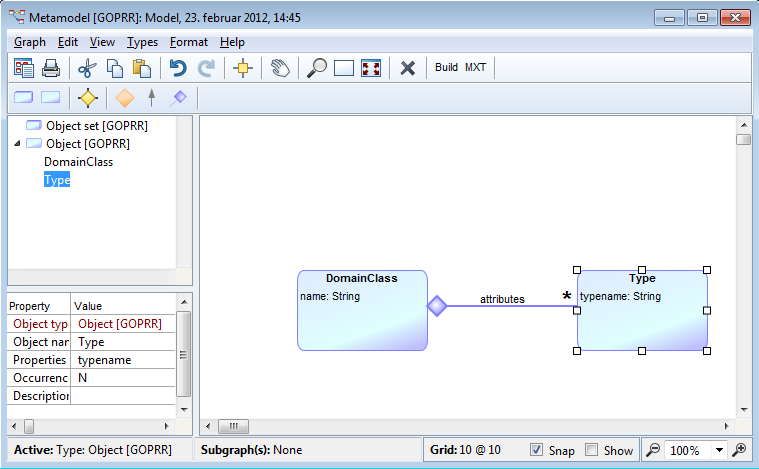
\includegraphics[scale=0.8]{images/me_mm_editor.png}}
  \caption[MetaEdit+ metamodel editor]{Figure shows the editor for metamodelling.}
  \label{fig:metacase_metamodel}
\end{figure}

Figure \ref{fig:metacase_metamodel} shows the editor where metamodels are created using \emph{GOPRR} which consists of the following modelling concepts~\cite{oprrmanual}:
\begin{description}
  \item[Graph] Specifies a modelling language.
  \item[Objects] This is the main type which is the node in the graphs. Used to model e.g. classes and states.
  \item[Object set] A collection of objects.
  \item[Property] This defines a property on a object. E.g name and ID.
  \item[Relationship] Connection between two or more objects. The relationships are connected to objects with roles. This is equivalent to an association in UML. 
  \item[Role] A role defines how an object behaves in a relationship. Each object in the relationship has a defined role. E.g. in an inheritance relationship, you have two roles: ancestors and descendants.
\end {description} 
GOPRR follows the four level hierarchy the same way Ecore does. You may model your system directly and "skip" a level, or specify another language. MetaCase includes a lot of languages for some more or less popular domains for reference and use. Among them we find DSMLs for insurance, UML, state machines, family trees, home automation etc.

\begin{figure}[hp]
  \centering
  \centerline{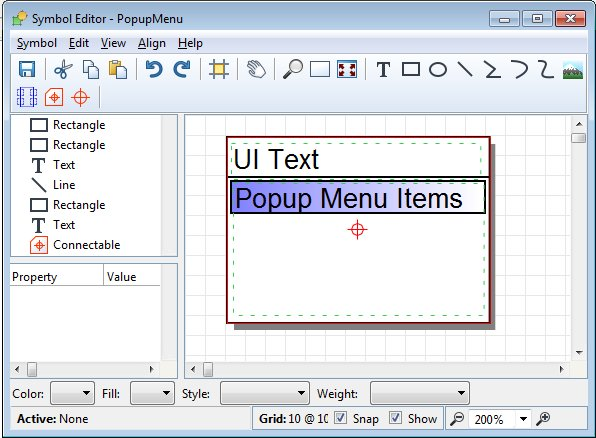
\includegraphics[scale=0.8]{images/me_symbol_editor.jpeg}}
  \caption[MetaEdit+ symbol editor]{Figure shows the editor for creating custom symbols.}
  \label{fig:metacase_symbol}
\end{figure}

One of the biggest features in MetaEdit+ is the ability to create custom symbols for the metamodel. These symbols can greatly improve the modelling experience for users of the DSML. Figure \ref{fig:metacase_symbol} shows the symbol editor where it is possible to draw a symbol or import graphics. This particular example shows a menu entry with a list of items in a Symbian Series 60 application DSML. The symbols can utilize particular aspects of the object entities.

\begin{figure}[hp]
  \centering
  \centerline{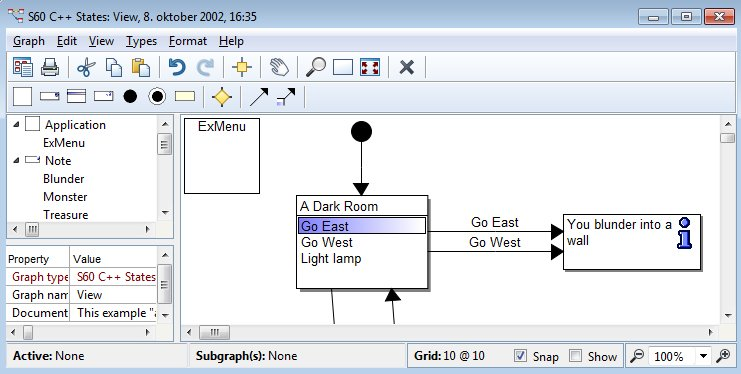
\includegraphics[scale=0.6]{images/me_instance_model_editor.jpeg}}
  \caption[MetaEdit+ instance model editor]{Editing an instance model of the Series 60 language in MetaEdit+.}
  \label{fig:metacase_metamodel}
\end{figure}

Figure~\ref{fig:metacase_metamodel} shows the creation of a Series 60 mobile application using the DSML defined in MetaEdit+. 

\begin{figure}[hp]
  \centering
  \centerline{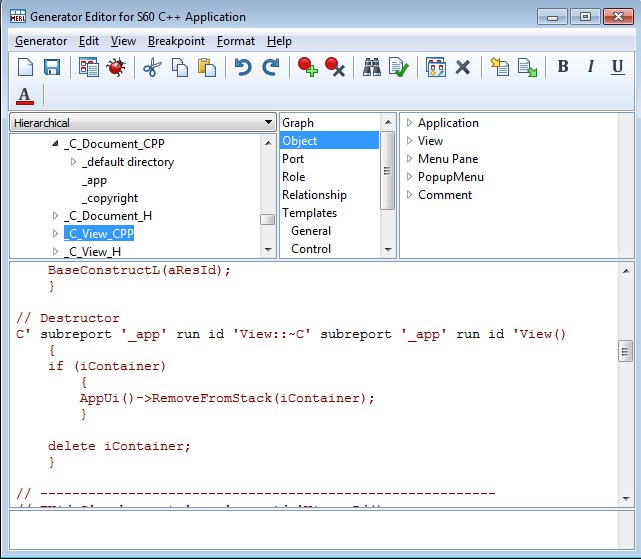
\includegraphics[scale=0.6]{images/me_template_editor.jpeg}}
  \caption[MetaEdit+ template editor]{Template editing in MetaEdit+.}
  \label{fig:metacase_template}
\end{figure}

Figure \ref{fig:metacase_template} shows the code generation template editor for the Series 60 example in \ref{fig:metacase_metamodel}. A metamodel can have several code generators associated with it.

Constraints in MetaEdit+ are created inside the model, which means that there is no support for \emph{attached constraints} (e.g. OCL). Unfortunately all constraints are pre-defined and there is no possiblity of creating custom constraints with corresponding symbol. All constraints are validated when modelling. A few of the pre-defined constraints include:
\begin{description}
  \item[Multiplicity]
  \item[Uniqueness]
  \item[Connectivity Constraints]
  \item[Explosions and Decomposition] \hfill \\
  A state in state diagram may be expanded into a separate diagram.
\end{description} 

The MetaEdit+ products are stand-alone proprietary software and is not built on Eclipse or similar platforms. It does however provide plug-ins for both Visual Studio and Eclipse with its new 5.0 release. MetaEdit+ supports Windows, Linux and Mac, but the latest beta release (which the illustrations are from) only supports Windows.

\section{Diagram Predicate Framework}\label{sec:dpf}
Diagram Predicate Framework (DPF) is an ongoing project at Bergen University College and the University of Bergen. The project started in 2006 with the aim to create a formal approach to MDE, with features as metamodelling, model transformations and model management. The framework is based on the Generalised Sketches formalism by Zinovy Diskin~\cite{DiskinKadish03}, and relies heavliy on mathematical concepts like category theory and graph transformations.

DPF facilitates a completely diagrammatic approach to MDE. DPF provides a multi-layer diagrammatic metamodelling hierarchy, where the need for attached constraints are removed. One of DPF's strengths is its general nature; it can be used as pattern to model other modelling language like UML, petri-nets and ER diagrams~\cite{RutleWolterL08TR367UIB}.

\begin{itemize}
  \item A DPF model consists of a \emph{specification $\spec{S}$} which consists of an underlying graph $S$, along with a set $\aconst{S}$ of \emph{atomic constraints $(\pi, \delta)$}.
%   \item A constraint $\pi \in \pred{\Sigma}$
  \item A signature $\sig{\Sigma} = \sigf{\Sigma}$ consists of a collection of predicate symbols $\pred{\Sigma}$.
  \item The constraints are instances of predicates $\pred{\Sigma}$.
\end{itemize}

A \emph{predicate} consists of a symbol, shape graph, visualization and a semantic interpretation. Predicates are defined within a \emph{signature}. Listing~\ref{list:multconstraint} shows the XML based definition of a multiplicity predicate. It defines a shape graph with two nodes and an arrow, a textual symbol \codeText{[mult(m,n)]}, and the semantic interpretation which is a Java based validator.

\lstset{language=xml,caption=A predicate for a multiplicity constraint.,label=list:multconstraint,captionpos=b}
\begin{table}[ht]
  \centering
  \begin{lstlisting}[showstringspaces=false]
<predicates symbol="[mult(m,n)]">
  <shape id="41921737-3a3a-4404-8d2a-a4ffe39da992" name="Default name">
    <nodes id="0867fde8-4eb6-4d42-be2d-715540a584d6" name="n_1"/>
    <nodes id="c4cce51b-3ab0-4e96-970a-18849131cbb3" name="n_2"/>
    <arrows id="554183df-2788-4469-ba63-84973bbb1d17" 
	target="//@predicates.10/@shape/@nodes.1" 
	source="//@predicates.10/@shape/@nodes.0" name="a_1"/>
  </shape>
  <semanticsValidator xsi:type="no.hib.dpf.core:MultiplicitySemantics"/>
</predicates>
  \end{lstlisting}
\end{table}

A central concept in DPF is graphs and graph homomorphisms. A graph homomorphism $\varphi$ is a mapping from a graph $G$ to another graph $H$, where the mapping preserves the source and target of each arrow. An atomic constraint $(\pi, \delta)$ in DPF consists of a predicate symbol as well as a graph homomorphism which defines what parts of the graph it constrains.

DPF defines two types of conformance relations which is \emph{typed by} and \emph{conforms to}. A meta-level $\spec{S}[i]$ is typed by the meta-level above $\spec{S}[i+1]$ if there is a graph homomorphism (also called \emph{typing morphism}) between the two meta-levels' underlying graphs: $\iota[i] : S[i] \rightarrow S[i+1]$. A specification $\spec{S}[i]$ at metalevel $i$ is said to conform to a specification $\spec{S}[i+1]$ at metalevel $i + 1$ if there exists a typing morphism $\iota[i] : S[i] \rightarrow S[i+1]$ such that $(S[i], \iota[i] )$ is a valid instance of $\spec{S}[i+1]$ ; i.e.  $\iota[i]$ satisfies the atomic constraints $\aconst{S}[i+1]$~\cite{dpf_editor_article}~\cite{rutle_thesis_2010}. See ~\cite{rutle_thesis_2010}~\cite{rossini_thesis_2011} for further discussions on DPF.

% A graph homomorphism consists of a pair of maps from the nodes and arrows of a graph to those of another graph, where the maps preserve the source and target of each arrow.
%  A specification Si at metalevel i is said to conform to a specification Si+1 at metalevel i + 1 if there exists a typing morphism ιi : Si → Si+1 such that (Si, ιi ) is a valid instance of Si+1 ; i.e.such that ιi satisfies the atomic constraints C Si+1 

% n DPF, two kinds of conformance relations are distinguished: typed by and conforms to. A spe-cification Si at metalevel i is said to be typed by aspecificationSi+1 at metalevel i + 1 if there exists a graph homomorphism ιi : Si → Si+1 , called the typing morphism, between the underlying graphs of the specifications. 
% - models are represented by diagrammatic specifications
% - specifications consists of a graph and a set of atomic constraints
% - Constraints are specifified in a predicates
% - predicates are defined in a signature
% - each predicate has an arity, a visualisation and a semantic interpretation
% - a dsl is a diagrammatic editor which consists of a signature and a metamodel
% -constraints and ocl\newline
% -grafhomomorfismar -> direkte typing frå ein node til ein anna node elns

\section{DPF Editor}

The DPF Editor is the reference implementation of DPF and its concepts~\cite{DPF_web}. There have been a few attempts the last years to implement earlier versions of DPF. The first attempt was performed by Ørjan Hatland in 2006~\cite{Hatland06}, a tool based on Microsoft .NET technology. This implementation was never completed and was not considered to be a good foundation for further development. In 2008, Stian Skjerveggen began the work on an Eclipse based solution~\cite{Skjerveggen08}. The core technology in this project was Graphical Modelling Framework (GMF)~\cite{GMP}, a framework that facilitates generation of graphical editors and tooling, based on EMF and Graphical Editing Framework (GEF). GEF facilitates creating rich graphical editors in Eclipse. This technology is somewhat "low-level", and requires a bit of work to achieve the same level of functionality which GMF can generate. GMF was at the end of the project deemed unsuitable for an implementation of DPF.

In 2010, Øyvind Bech and Dag Viggo Lokøen started the work on the current implementation of DPF, the DPF Editor~\cite{Bech11}. It is written from scratch using EMF and GEF and supports the most essential features concerning metamodelling:

\begin{itemize}
  \item Graph based projectional editing of models
  \item Storing/loading the models as XMI
  \item Arbitrary number of metalevels
  \item Checks typing between metalevels if there exists a graph homomorphism
  \item Checks constraints between metalevels
  \item Creation of predicates and corresponding Java validators
  \item Different simple symbols on nodes (circle, ellipse, rectangle etc.)\footnote{The creation of predicates and visualizations are later work by Ph.D. student Xiaoliang Wang.}
\end{itemize}
% \footnotetext[2]{The creation of predicates and visualisations are later work by Ph.D. student Xiaoliang Wang.}

None of the previous attempts to create DPF based software has reached a level of maturity where facilitating code generation was considered. 

\begin{figure}[htpb]
  \centering
  \centerline{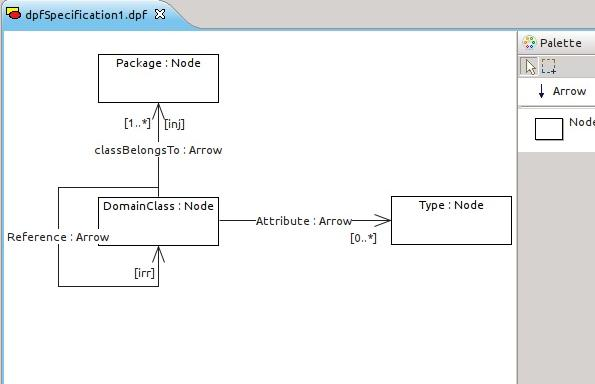
\includegraphics[scale=0.6]{images/dpf_editor.jpeg}}
  \caption[DPF Editor]{Creating a DSML in the DPF Editor.}
  \label{fig:dpf_editor}
\end{figure}

Figure~\ref{fig:dpf_editor} shows the editor view in the DPF Editor. We start off with only \codeText{Node} and \codeText{Arrow} when creating a DSML. The figure depicts a simple language for creating domain classes in web application. This model forms the basis for the tool demonstration i chapter~\ref{chap:case_study} and will then be explained further. Figure~\ref{fig:dpf_hierarchy} shows a subset of the DSML in figure~\ref{fig:dpf_editor} and how the different metalayers are typed by each other. The dotted lines shows conformance between the types levels.

\begin{figure}[htpb]
  \centering
  \centerline{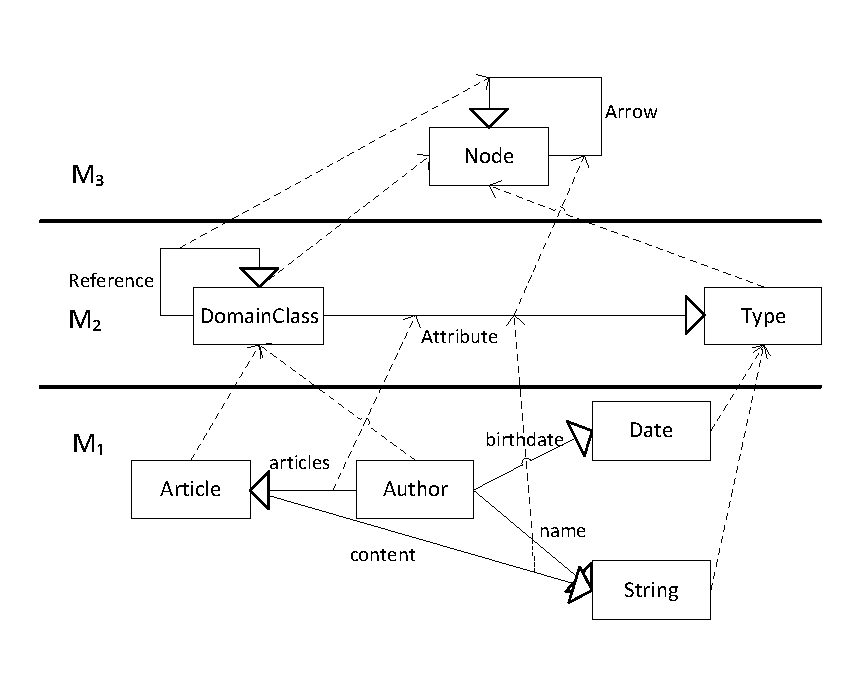
\includegraphics[scale=0.8]{images/dpf_hierarchy.pdf}}
  \caption[DPF DSML example]{Shows how the different DPF layers of a simple domain class DSML conforms to each other.}
  \label{fig:dpf_hierarchy}
\end{figure}

% The DPF Editor is under heavy development with the addition of new functionality all the time.
% [bilete av editor med model]
% [teikna eit hierarki elns]
% [bilete av predicat editor]
% [Klassediagram som viser dpf metamodell?]
% \begin{itemize}
%   \item Illustration showing the tool
%   \item Graphic editing of models
%   \item Metamodelling and typing of specifications
%   \item Constraints
% \end{itemize}
\newpage
\section{Comparison}
The evaluated tools has its strengths and weaknesses from a language workbench point of view. The concept of a language workbench is a pragmatic one, and this emphasizes usability of the tools. Even though EMF, Obeo Designer and MetaEdit+ are all mature products with a lot of users, they do not necessarily do everything right. A common problem is messy unintuitive user interfaces which significantly raises the bar for learning the software. 

The most complete (and most mature) tool, is MetaCase's MetaEdit+. It supports a wide variety of pre-defined popular modelling languages, but also has its own schema definition language, GOPRR. Obeo Designer improves on the shortcomings of plain EMF, with the possiblity of creating custom visualizations and support for code generation on the model level with Acceleo. Table~\ref{tab:lw_features} shows that a common trait between the three evaluated solutions; all support different forms of projections. The \emph{Projection Types} row use capital letters for describing a projection type:
D for diagrammatic, H for hierarchy, M for matrix and T for table.

Of the reviewed solutions we see that only the DPF Editor provides multi-level metamodelling, while the other adheres to the levels of MOF. As described, all three reviewed tools have a fixed number of metalevels. The metalevels may vary, because one can define e.g. UML through MOF's modelling facilities as shown in figure~\ref{fig:mof}. When it comes to constraints, we see that EMF only have support for \emph{structural constraints} inside the model and is dependent on external functionality for more advanced constraints. Since Obeo Designer is built around EMF, the same applies. MetaEdit+ has, like the DPF Editor, support for more advanced constraints within the model. There is however no option for defining constraints like in the DPF Editor, as they are fixed.

The DPF project can learn from other tools as there is a lot of room for improvement. The lessons learned are both good and bad; the tools studied all have usability issues, mostly related to complicated user interfaces. Having to use OCL for constraints also complicates the modelling process. Ideas like the symbol editor and multiple ways of projecting the model are some of the interesting features which the other tools more or less provide. 

A "projection" which none of the tools provide, are textual representation of the models (beyond serializing). The \emph{Language Workbench Competition (LWC)} which is a part of the \emph{Code Generation}~\cite{lwc} conference, refers to a language workbench that supports both diagrammatic and textual representation of a model as "the one language workbench to rule them all"\footnote{Florian Mantz has created a textual version of DPF in his Ph.D. thesis work. This work is currently not integrated with the DPF Editor.}. 

\let\Oldarraystretch\arraystretch
\renewcommand*\arraystretch{1.5}

\begin{table}[htb]  
  \flushleft
  \resizebox{1\textwidth}{!}{
    \begin{tabular}{|p{34mm}|p{26mm}|p{30mm}|p{22mm}|p{23mm}|}
      \hline
      \textbf{Tool}                   & \textbf{EMF}  & \textbf{Obeo Designer}  & \textbf{MetaCase MetaEdit+} & \textbf{DPF}\\
      \hline
      \textbf{Schema~Definition
	  \newline Language}          & Ecore                  & Ecore                             & GOPRR                    & DPF \\
      \hline
      \textbf{Symbol Editor}          & No                     & No                                & Yes                      & No \\
      \hline 
      \textbf{Projection
	\newline Types}               & D/H\footnotemark       & D/H/M/T                           & D/H/M/T                  & D \\
      \hline
      \textbf{Code~Generation
	\newline Facility}            & Yes\footnotemark       & Yes (Acceleo)                     & Yes                      & No \\
      \hline
      \textbf{Multi-level 
	\newline metamodelling}       & No                     & No                                & No                       & Yes \\
      \hline
      \textbf{Constraints}            & OCL                    & OCL                               & Model-based/Fixed        & Model-based/Custom \\
      \hline
      
    \end{tabular}
  }
%    \scalebox{0.77}{
%     \begin{tabular}{|p{26mm}|p{34mm}|p{25mm}|}
%       \hline
%       \textbf{Tool}                   & \textbf{Multi-level metamodelling}  & \textbf{Constraints}  \\
%       \hline
%       \textbf{EMF}                    & No                        & OCL                     \\
%       \hline 
%       \textbf{Obeo Designer}          & No                        & OCL                     \\
%       \hline 
%       \textbf{MetaCase MetaEdit+}     & No                        & Model-based/Fixed      \\
%       \hline
%       \textbf{DPF}                    & Yes                       & Model-based/Custom     \\
%       \hline
%     \end{tabular}
%   }
  \caption {Language workbench features}
  \label{tab:lw_features}
\end{table}
\footnotetext[4]{EMF provides a diagrammatic view for the metamodel, but not for the models.}
\footnotetext{EMF generates editors and code for your metamodel, but does not facilitate code generation from the instance model.}
% template language, profiler, template editor, custom generator metamodel, 
\let\arraystretch\Oldarraystretch



